\documentclass[12pt,english]{article}
\usepackage{mathptmx}

\usepackage{color}
\usepackage[dvipsnames]{xcolor}
\definecolor{darkblue}{RGB}{0.,0.,139.}

\usepackage[top=1in, bottom=1in, left=1in, right=1in]{geometry}

\usepackage{amsmath}
\usepackage{amstext}
\usepackage{amssymb}
\usepackage{setspace}

\usepackage[authoryear]{natbib}
\usepackage{url}
\usepackage{booktabs}
\usepackage[flushleft]{threeparttable}
\usepackage{rotating}
\usepackage{graphicx}
\graphicspath{ {./images/} } % enable on upload
\usepackage[english]{babel}
\usepackage{pdflscape}
\usepackage[unicode=true,pdfusetitle,
 bookmarks=true,bookmarksnumbered=false,bookmarksopen=false,
 breaklinks=true,pdfborder={0 0 0},backref=false,
 colorlinks,citecolor=black,filecolor=black,
 linkcolor=black,urlcolor=black]
 {hyperref}
\usepackage[all]{hypcap} % Links point to top of image, builds on hyperref
%\usepackage{breakurl}    % Allows urls to wrap, including hyperref
\usepackage{indentfirst}
\linespread{2}

\begin{document}

\begin{singlespace}
\title{Exploring Strava's Suffer Score}versity of Oklahoma.\
E-mail~address:~\href{mailto:saryu@ou.edu}{saryu@ou.edu}}}

% \date{\today}
\date{April, 2023}

\maketitle

\begin{abstract}
\begin{singlespace}
Training load quantification is a method of assessing the physiological impacts of a given workout. This kind of metric can provide coaches and athlete with valuable insights to how an athlete is responding to a prescribed workout. However, it is difficult to integrate into the decision making process as ease of access can be an issue. This project aims to estimate Strava's suffer score (a metric that quantifies training load) by using widely available activity summary metrics and the multiple linear regression model. To construct a viable multiple linear regression model, the backwards step-wise method of variable selection was used. This project found that by utilizing quadratic data transformation and interaction terms, a linear model would be able to estimate suffer score moderately well (Adjusted R-squared = 0.8). Hence this method of sufance metric that represents how tough an act measures of training load \cite{bourdon2017monitoring}. According to \cite{StravaSufferScore}, their  based on time spent in various heart rate (HR) 'zones'. The time spent in a higher HR zone is weighed heavier, comptime spent in a lower HR zone. Despite this measure being re-branded to "Relative Effort" (RE) recently, it will be referred to as sutraining load metric using simpler activity summary metrics to improve access, whether that may be for new users who are curious or athletes who do not h===============================
\section{Literature Review}\label{sec:litreview}
The term "training load" is often used in exercise physiology to describe a typenk about exercise and their adaptations as a "dose-response" relationship, where exercise provides a dose of physiological stress that our body responds to, through training adaptaticite{paquette2020}, they describe this metric in great detail. The authors explain that training load is defined as a product of external and internal load. External load is tare typically measures of time, distance or speed but can include others like ground reaction forces. Internal load is the physiological stress response that occurs due to the external eived exertion (RPE). By calculating the product of these two types of measures, the training load takes both mechanical and physiological stresses applied to the body. In a way, this caivity. 

In a review article, \cite{lambert2010measuring} discuss the concept of quantifying training load, as well as the various methods used to quantify training  quantified, and there is no "gold standard" that has been formally established. Different methods have various advantageous and disadvantageous. For example, lab equipment can be used to meata. However, these methods can be highly impractical for everyday use due to the cost and portability of the  equipment. Other methods discussed include TRIMP, modified TRIMP and session RPE. The agths and weaknesses, some are more desirable over others. The method that is most often used among the this list is TRIMP.  is an abbreviation of training impulse, and is a method of quantifying training load developed in the early 1990s as lht and reliable heart rate monitors started to become available comercially. 

Although the quantification of training load is accepted as an essential parton amongst practitioners and athletes. In an article by \cite{roos2013monitoring}, the authors conducted several focus groups with elite coion of training load. In this, Roos et al. found that many coaches agreed that monitoring an athlete’s physical condition in response to trainning good quality data from athletes at a consistent rate and 2) being able to respond to this data at promptly. To overcome these challenges, the coaches in the focus groups discussed the importance of feasibility of the  distrust in the measure was not the issue. Instead, the concern was the ease of use when it came to utilising training load monitoring. 

Strava's suffer score can be seen as one way to make mea one way to quantify training load, it appears to use techniques similar to the TRIMPS method, using heart rate and duration as two of the main components \cite{S with the current standards of training load quantification in exercise physiology. Hence, this could be considered as a metric that coaches and athletes can integrate into their repertoire, when assessing physiological===================================
% Data
%=========================================
\section{Data}\label{sec:data}
Data used in this project comes from Strava activity logs. Because Strava is arecord of all uploaded activities. The data is mostly numerical and consist of summary metrics of the activities. This includes duration, distance, speed, elevation ms, and power averages and maximums are also present. These depend on whether the user utilizes technology such as heart rate monitors and power meters.

In as, social interaction metrics (kudos and comment count) and foreign keys for gear selection (if recorded), maps, and the activity stream. eatures. This a separate data table is tied to the activity log data through the activity stream foreign key (activity ID). 

\subsection{Data Collection}
Data for this project was scraped from the activity log of a single and the rStrava R package. The data was then loaded into R studio software for further analysis. There are a few reason why data was only collected from one user. Firstly users. Each request for data prompts the target user to authenticate the access. Hence, it was most practical to use a single user profile that was easily access to exercise can drastically differ between individuals and environmental conditions. Because physiological responses to exercise will be the mainsers was not imperative to meet the goals of this specific project.

%========================================
% Methods
%========================================
\section{Methep-wise multiple regression, with the goal of analyzing the magnitude of impact of relevant metrics on the Suffer Score. The multiple regression model can be depicted by the following equation:

\begin{equation}
\label{eq:1}
Y_r=\beta_{0} ++ \beta_{2}X_{2} + ... + \varepsilon,
\end{equation}

For this project, $Y_r$ represents the Strava Suffer Score for recorded runs ($r$), and nfluence each metric has towards estimating the Suffer Score. 

\subsection{Data Cleaning}
Before the analysis, the activity log was filtered to only include summary metrice the goal of the project was to determine what summary metrics could be used make the best estimation the Suffer Score. The data was also filtered to o this data set) can differ significantly \cite{hassmen1990perceptual}. Finally, the data was filtered to only include runs that had heart rate  and Strava would not have generated a Suffer Score in the absence of heart rate data.

The data was then mutated. First, some of the data had to be co analysis method. Additionally, the time variable was converted from time in seconds, to time in minutes. This was done to make the data easily understandable and user friendly.

egression was conducted. The general method of this started with creating a linear model with all the available variables. This initial model is then put through the process of v In R, this was done using the lm() function for the initial regression, and the step() or stepAIC() functions for the step-wise regression. 

In the project, three mainforward backwards step-wise multiple regression in which no variables were manipulated. The next model was an extension of the first model, with added quadratic terms. The final model was erms between a time or distance and heart rate or cadence.   

%========================================
% Results
%========================================
\section{Research Findings}\label{sec:results}
The data used in the models are summarized in table \ref{tab:descriptives}. There were 306 observations in the final data set and the mean th a mean of 47.7. The models were summarized in table \ref{tab:estimates}, in order of complexity. 'model 1' is the standard backwards step wise multiple regression, 'model 2' includens. 

The most significant predictors of suffer score appears to exclude  elevation gain in all three models. For the first model, the only predictors included in thnificant (p$<0.05$). Model 2 excludes distance, but includes maximum heart, in addition to the quadratic terms of distan, speed and heart rate (p$<0.05$). Model 3 includes 13 predictors. 6 of these are simple su and the remaining 4 are interaction terms between distance/time and heart rate/cadence.

The summary of the three models (Table \ref{tab:estimates}) show that the most complex  outcome variable Suffer Score to a greater level of accuracy (adjusted R-squared of 0.8 and RMSE of 14.65). With that said, the least accurate model ictions of the models were plotted against the actual suffer score values, these performance differences can be put into context. The performance lues and the y axis contains the actual suffer score values. The prediction accuracy gets increasinglvalues increase. This indicates high heteroscedasticity, or varying error depending on the value. Furthermore, many negative suffer scores are predicted, which are invalid predictions. 

Figure \ref{fodel 1, model 2 has achieved some improvements, particularly, at higher values. This is signified by the tighter distribution of points ajusted R-squared values and RMSE values indicate that model 3 has the best performance. This is visually demonstrated in figure \ref{fig:fig3}. Predictions are fairly consistent from low to high values. Althoill present, it is to a lesser degree, compared to the previous models.

%========================================
% Conclusion
%========================================
\sectsuffer score has demonstrated the limits of utilizing simple activity summary metrics and linear regression methods to accurately estimate sechnique, or integrates more in-depth data from activity streams to calculate their suffer score. With that said, the model predictions were not too far of the actual suffer score. The analysions, and interaction terms between some of the summary metrics, a linear model can account for approximately 80\% of the variation.

Ultimately, Strava's suffer score is only one version ohis metric is highly individual and open to interpretation. There are no clear ties between our physiological condition and the suffer score, that has been shown in scientific literamay be sufficient, as it could satisfy their curiosities of the suffer score metric. 

For future research, the model developed in this project could be tested with dataditionally, machine learning and the activity stream data could be integrated to generate a model that may estimate Suffer Score better. However, more interesting researcining load quantification to subjective measures like fatigue and rate of perceived exertion, and physiological markers of stress.

\vfill
\pagebreak{}
\begin{spacing}{1.0}
\bibliographystyle{jpe}
\bibliography{references.bib}
\addcontentsline{toc}{section}{References}
\end{spacing}

\vfill
\pagebreak{}
\clearpage======================================
\section*{Figures and Tables}\label{sec:figTables}
\addcontentsline{toc} and Tables}

%----------------------------------------
% Table 1
%--------------------caption{Statistics for Strava Run Data}
\label{tab:descriptives} 
\centering
\be&\\
\multicolumn{7}{l}{}\\
\toprule
Metric (units)  & Unique (\#) & Mean & SD & Min & Median & Max\\
\midrule
suffer\_score & 110 & 47.7 & 33.5 & 2.0 & 42.0 & 208.0\\
distance & 341 & 11.4 & 4.6 & 0.9 & 11.0 & .5 & 58.0 & 44.7\\
average\_speed & 306 & 12.4 & 1.6 & 8.4 & 12.4 & 20.2\\
total\_elevation\_gain & 281 & 54.9 & 59.7 & 0.0 & 36.2 & 303.1\\
average\_heartrate & 239 & 147.6 & 11.8 0 & 204.0\\
average\_cadence & 83 & 88.1 & 2.2 & 76.8 & 87.8 & 97.5\\
\bottomrule
\end{tabular}
\footnotesize  for all variables is $N=306$.
\end{threeparttable}
\end{table}


%----------------------------------------
-------------------------------
\begin{table}[ht]
\caption{Model Summaries}
\label{tab:estimates} 
\centering
\begin{threepartble}
\begin{tabular}{lccc}
%&&&&\\
\multicolumn{4}{l}{}\\
\toprule
  & model 1 & model 2 & model 3\\
\midrule
(Intercept) & {-213.131}*** & {-177.770} & {158.134}\\
 & ({<0.001}&  & ({0.732})\\
time\_minutes & {-0.599}*** & {0.711}*** & {-9.337}*\\
 & ({<0.001}) & ({<0.001}) & ({0.042})\\
average\_heartrate & {1.430}*** & {9.855}*** & {11.070}***\\
 8}***\\
 &  & ({<0.001}) & \vphantom{2} ({<0.001})\\
I($distance^2$) &  & {0.205}*** & \\
 &  & ({<0.001}) \vphantom{1} & \\
I($time\_minutes ({0.003})\\
I($average\_heartrate^2$) &  & {-0.028}*** & {-0.035}***\\
 &  & ({<0.001}) & \vphantom{1} ({<0.0rtrate^2$) &  & {0.024}*** & {0.021}***\\
 &  & ({<0.001}) & ({<0.001})\\
average\_speed &  &  & {-18.419}*\\
 &  &  & ({0.011})\\
average\_cadence &  &  & {-3.986}***\\
 &  &  & \vphantom{3} ({<0.001})\\
distance × average\_heartrate &  &  & {0.440}***\\
 &  &  & \vphantom{2} ({<0.001})\\
distance × average\_cad_heartrate &  &  & {-0.066}***\\
 &  &  & \vphantom{1} ({<0.001})\\
time\_minutes × average\_cadence &  &  & {0.214}***\\
 &  &  & ({<0.001})\\
\midrule
%Num.Obs. & {343} & {343} & {343}\\
%R2 & {0.710} & {0.738} & {0.808}\\
R2 Adj. & {0.708} & {0.732} & {0.801 {-1407.439}\\
%F & {277.181} & {117.876} & {106.620}\\
RMSE & {18.00} & {17.11} & {14.65}\\
\bottomrule
\end{tabular}
\footnotesize Notes:{\rule{0pt}{1em}+ p ---------------------------------
% Figure 1
%----------------------------------------
\begin{figure}[ht]
\center%includegraphics[width=.9\linewidth]{model1}
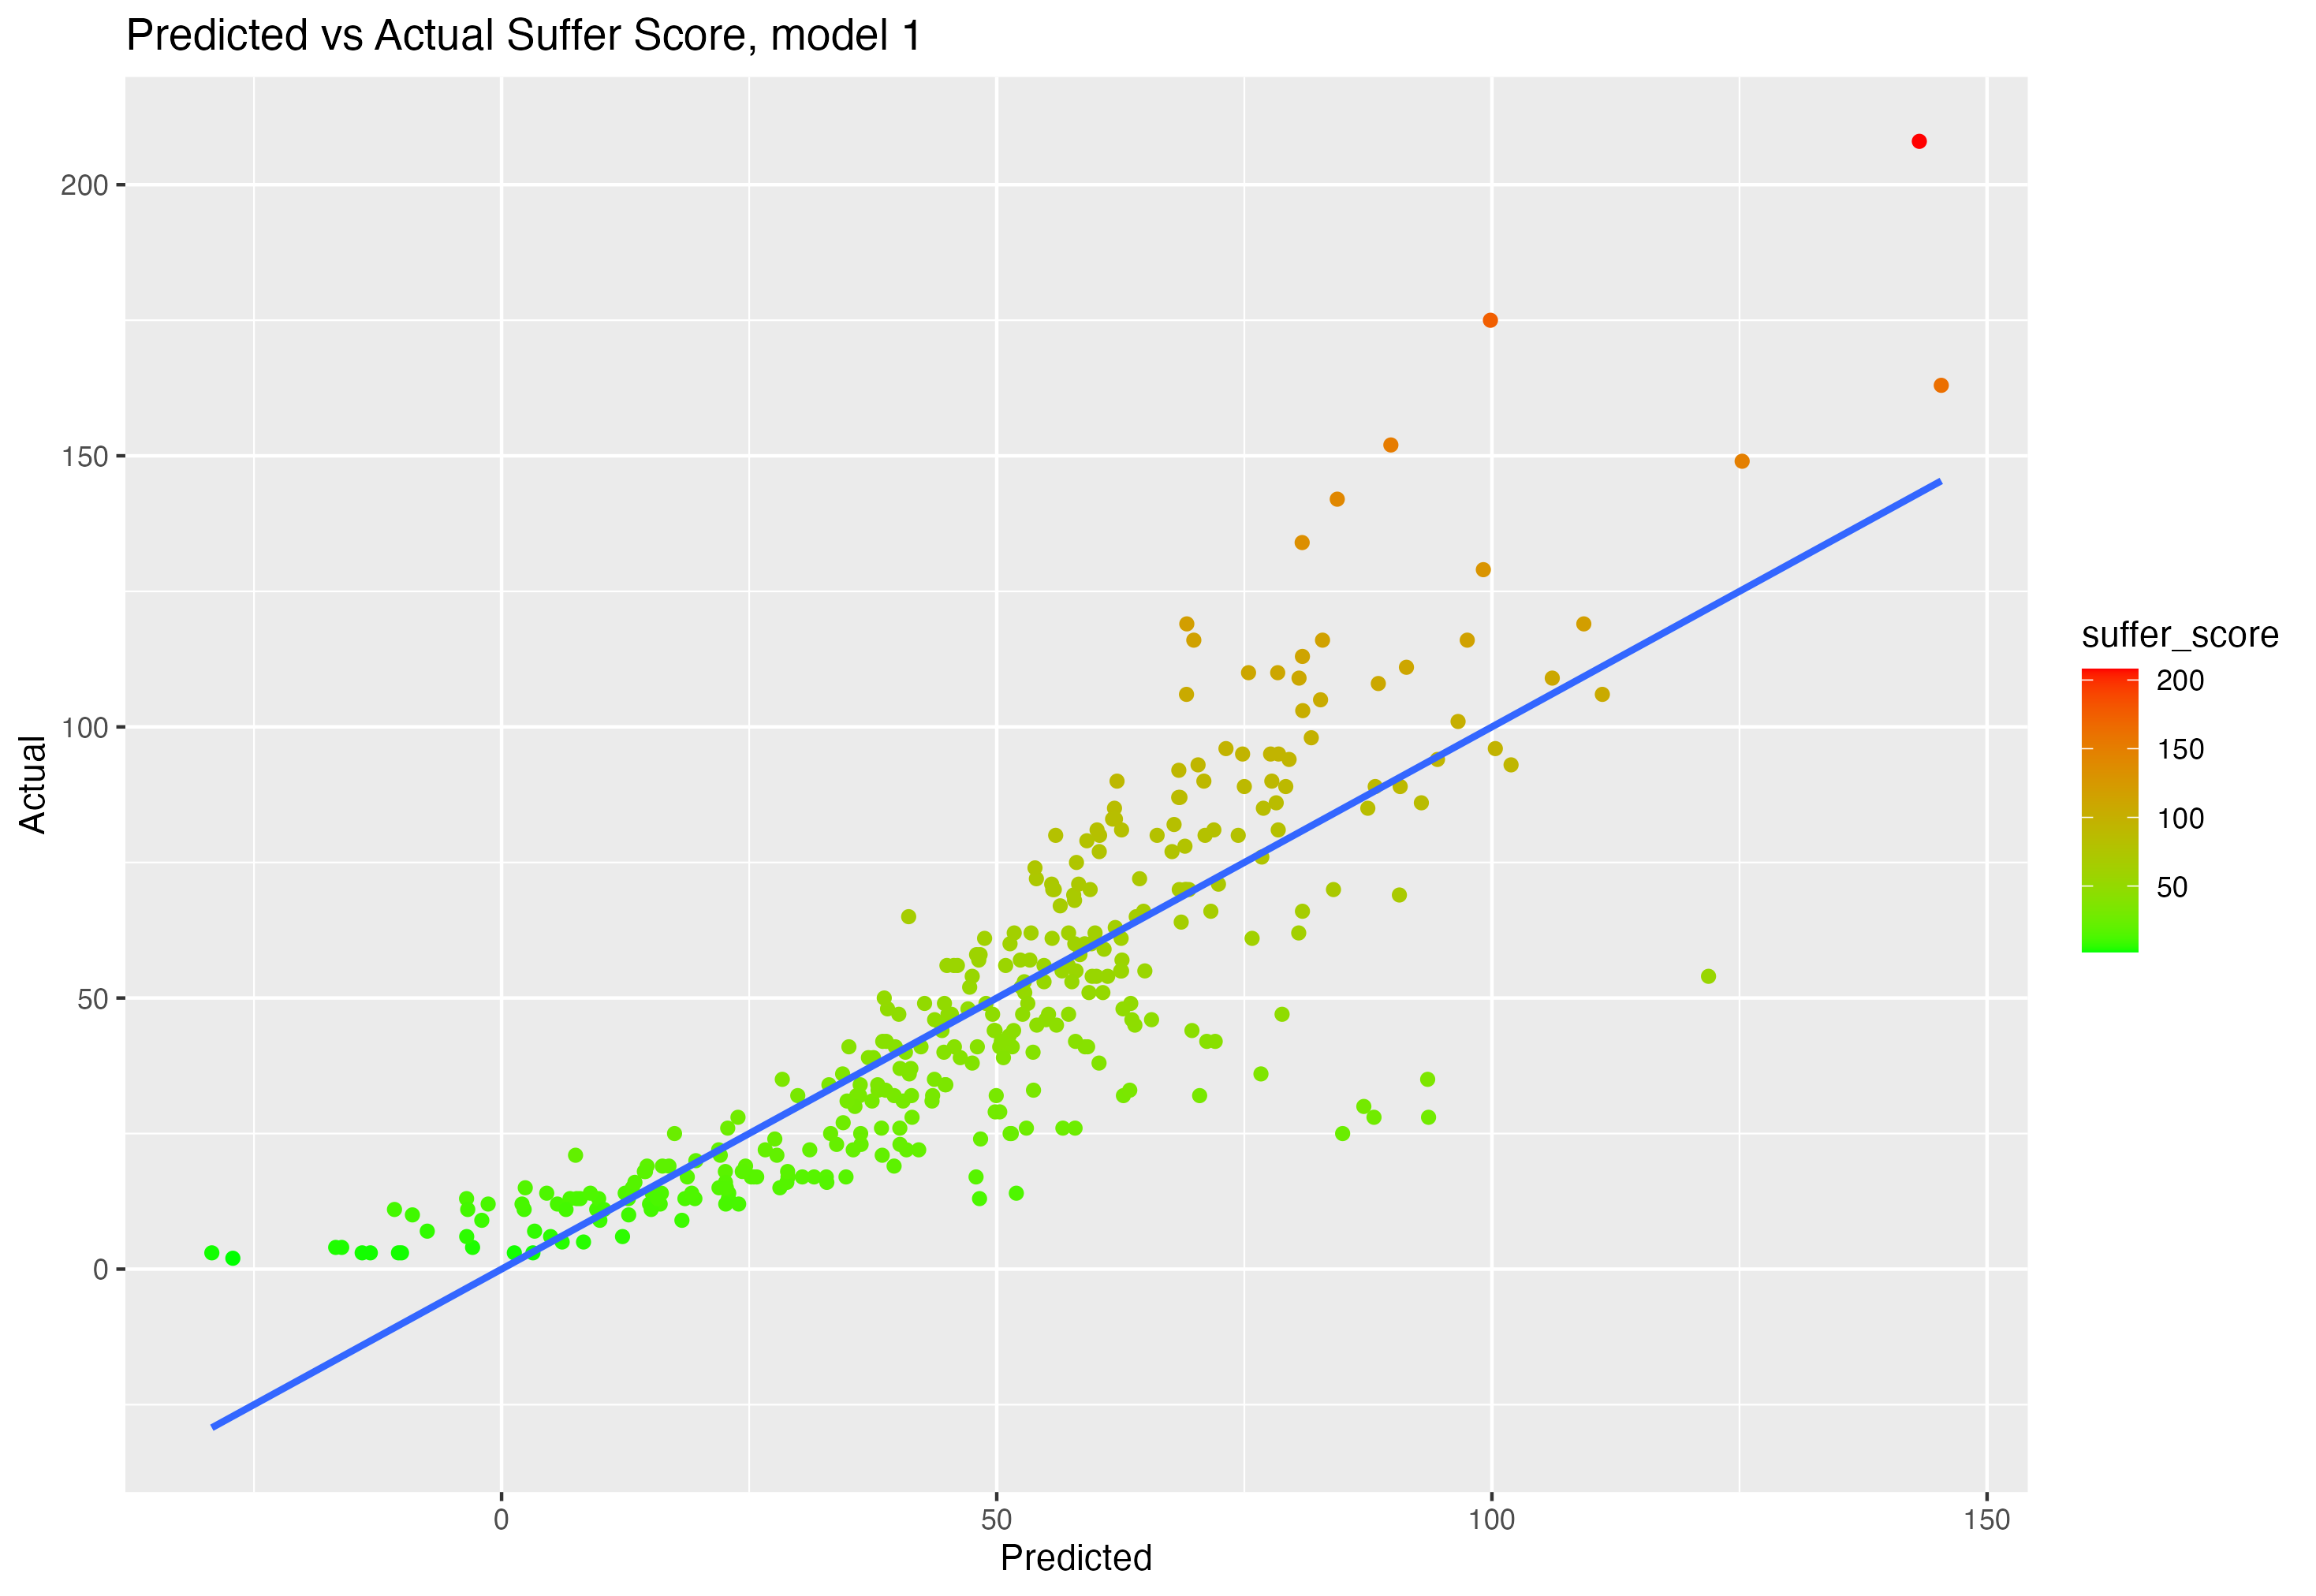
\includegraphics[width=12cm]{model1.png}
\caption{Predictions of Model 1}
g:fig1}
\end{figure}

\begin{figure}[ht]
\centering
\bigskip{}
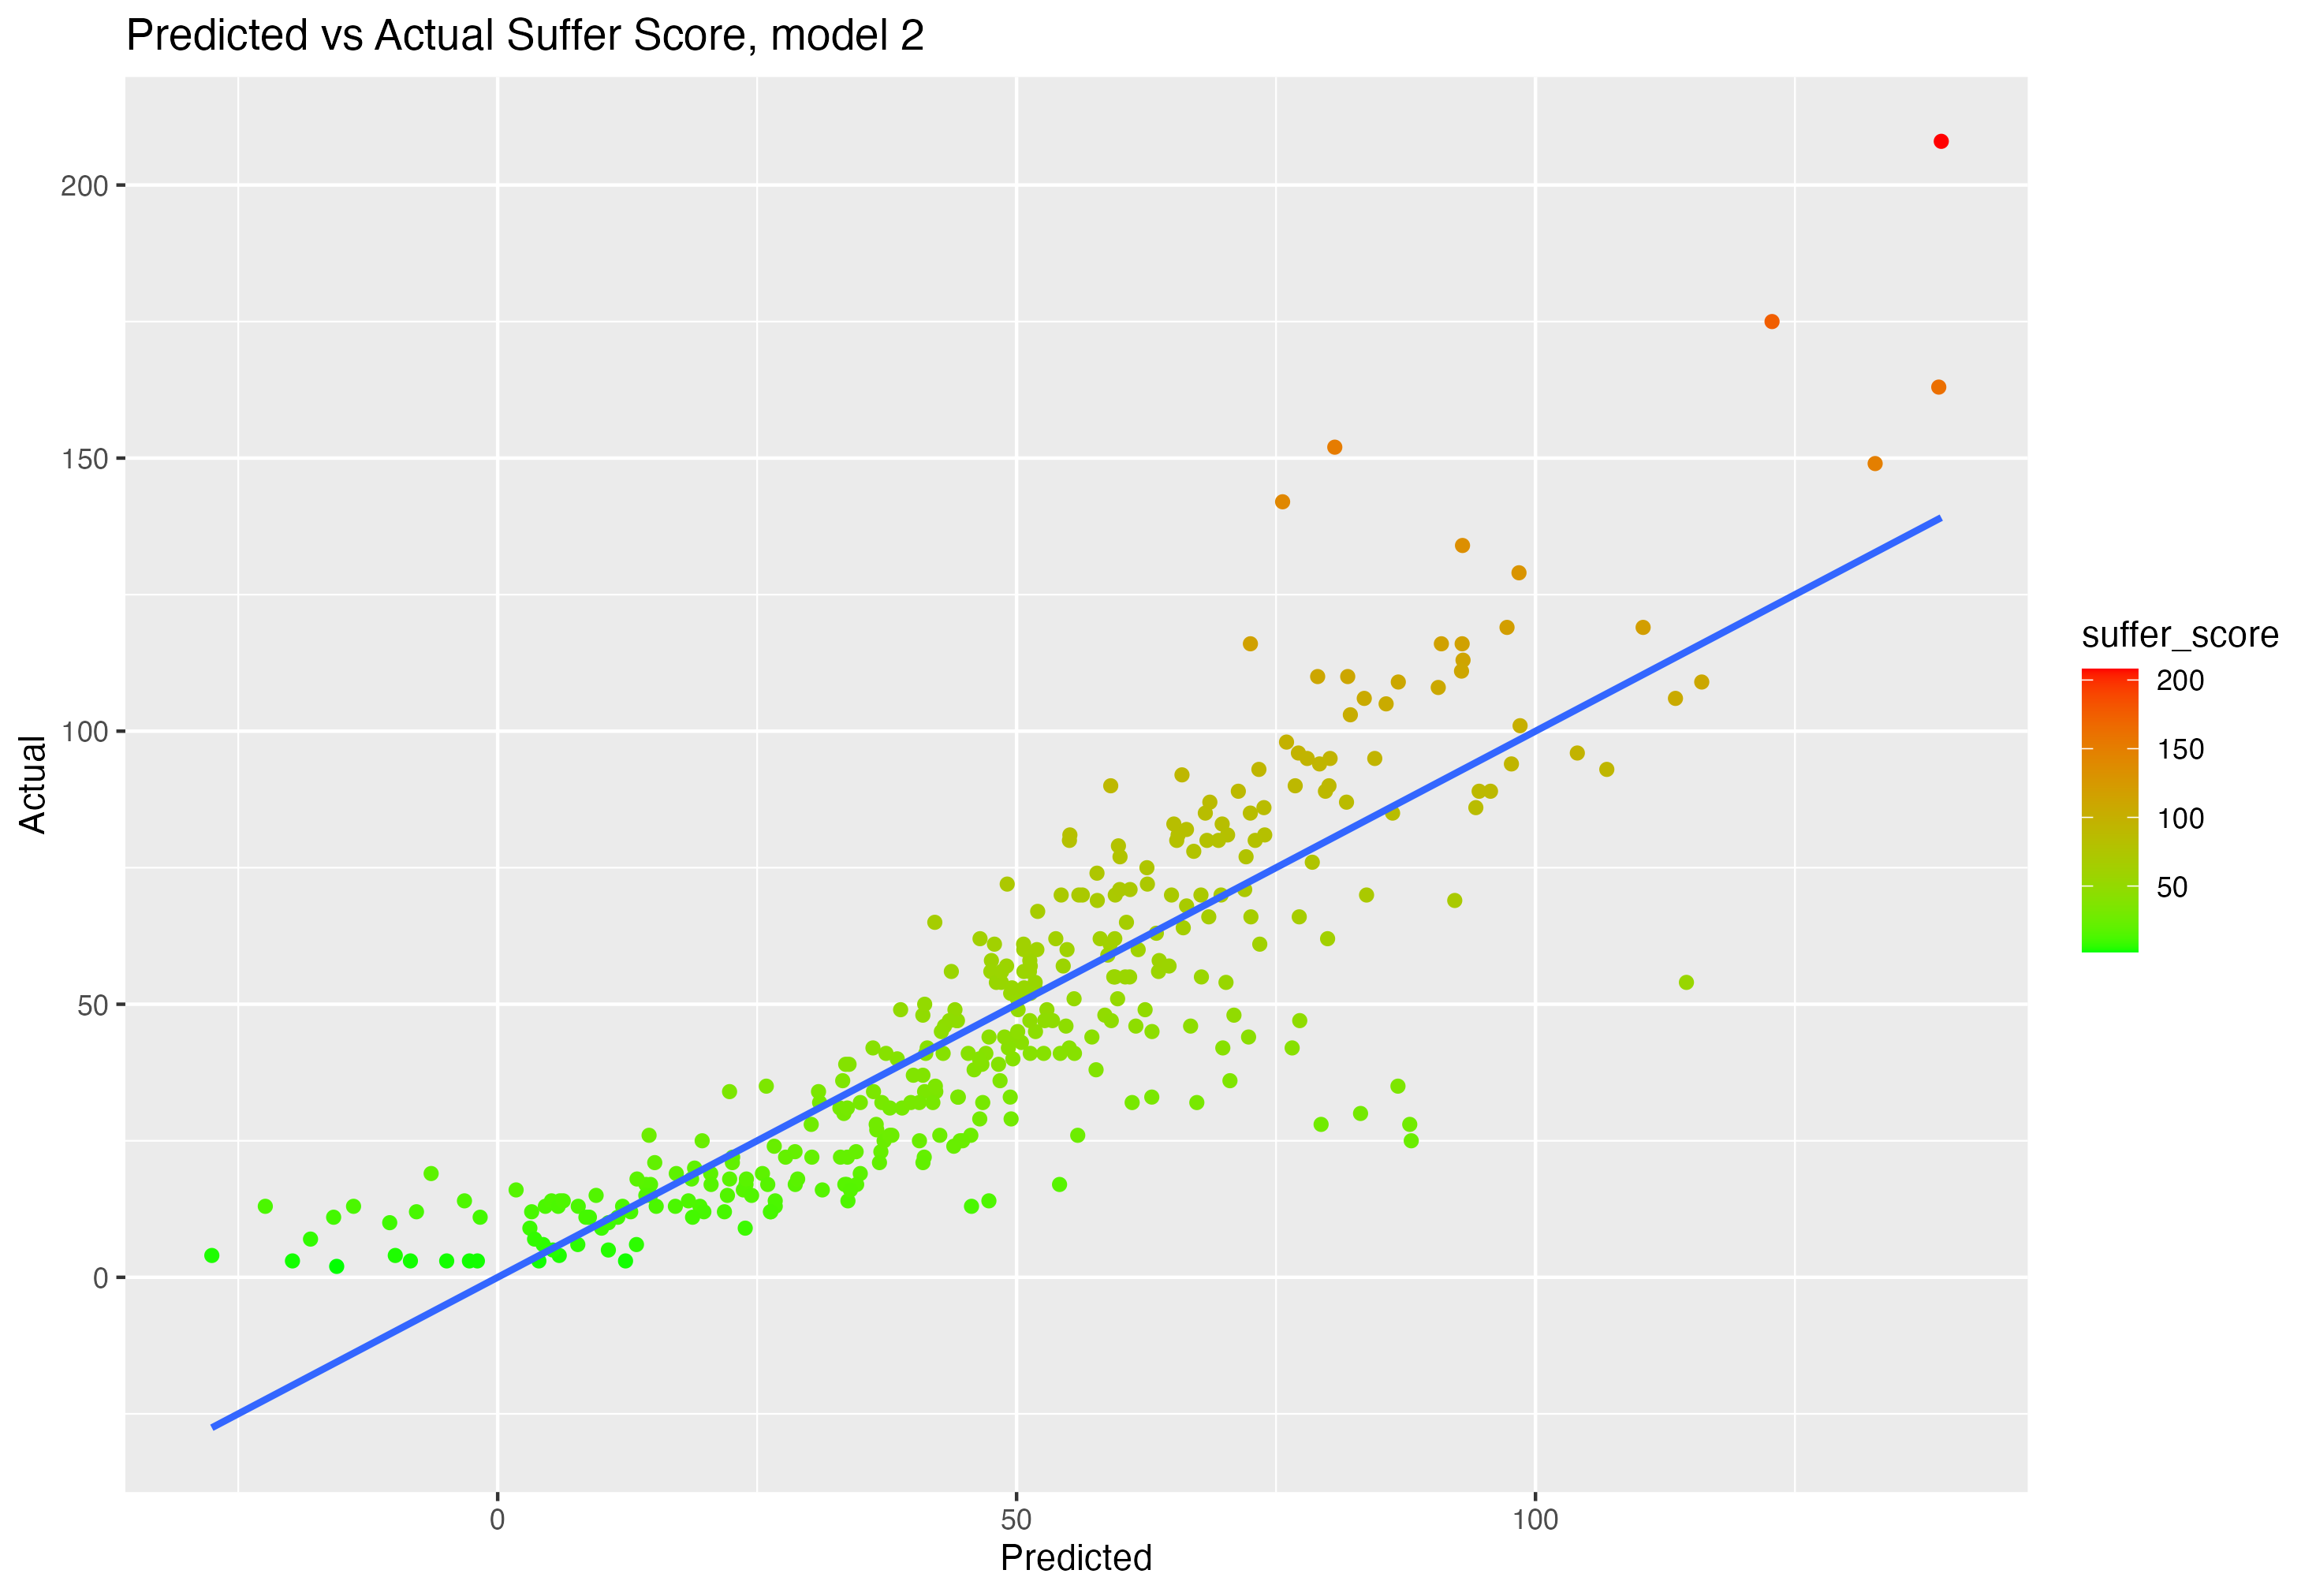
\includegraphics[width=12cm]{model2.png}
\caption{Predictions of Model 2}
\label{on{Predictions of Model 3}
\label{fig:fig3}
\end{figure}

\end{document}

